\documentclass[a4paper, 12pt]{report}

\usepackage[latin1]{inputenc}
\usepackage[T1]{fontenc}
\usepackage[sc]{mathpazo}
\usepackage[english]{babel}
\usepackage{graphicx}
\usepackage{color}
\usepackage{array}
\usepackage[margin=2.5cm]{geometry}
\usepackage{hyperref}
\usepackage{enumitem}
\usepackage{float}
\usepackage{amsmath}
\usepackage[labelfont=bf]{caption}
\usepackage{algorithm}
\usepackage[noend]{algorithmic}
\usepackage{setspace}


\usepackage{blindtext}
\usepackage[ttdefault=true]{AnonymousPro}

\usepackage[toc, page]{appendix}

\usepackage{standalone}

\usepackage{listings}

\usepackage{cleveref}
\crefname{section}{\S}{\S\S}
\Crefname{section}{\S}{\S\S}


% listings
\definecolor{deepblue}{rgb}{0,0,0.5}
\definecolor{deepred}{rgb}{0.6,0,0}
\definecolor{deepgreen}{rgb}{0,0.5,0}

\lstdefinestyle{mystyle}{  
    commentstyle=\color{deepgreen},
    keywordstyle=\color{deepblue},
%    numberstyle=\tiny\color{codegray},
    stringstyle=\color{deepred},
    basicstyle=\footnotesize,
    breakatwhitespace=false,         
    breaklines=true,                 
    captionpos=b,                    
    keepspaces=true,                 
    numbers=left,                    
    numbersep=5pt,                  
    showspaces=false,                
    showstringspaces=false,
    showtabs=false,                  
    tabsize=2,
    frame=shadowbox
}
 
\lstset{style=mystyle}

% math 
\newcommand\floor[1]{\lfloor#1\rfloor}

\newcommand{\skippage}{\newpage\null\newpage}

\newcommand*{\titleTH}{ % title page
\begingroup
\raggedleft
\thispagestyle{empty}
{\Large Pavel Berkovich}\\[0.167\textheight] \centering
{\huge \texttt{N0NaMe\_}}\\[\baselineskip]
{\Large Peer-to-peer conversation security \\ using KleeQ} \\
\begin{figure}[h]
    \centering
    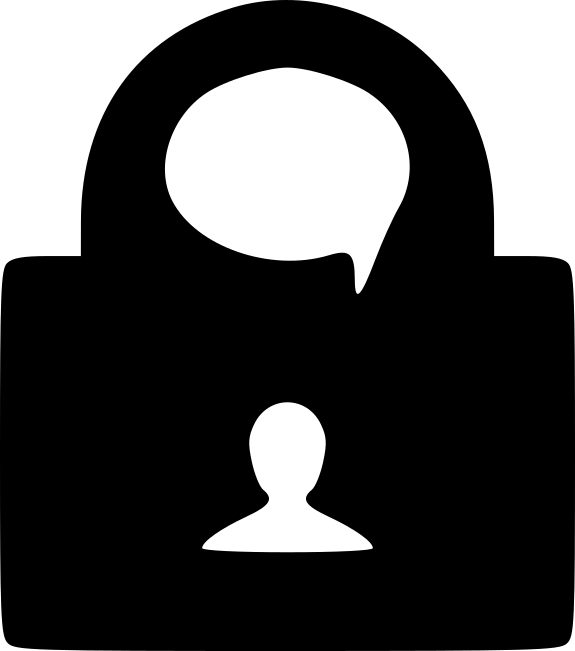
\includegraphics[width = 0.8\textwidth]{lock_chat.png} 
\end{figure}
{\large Computer Science Tripos, Part II}\\ \vspace{3mm}
{\large St John's College} \\ \vspace{3mm}
{\large 13th May, 2016}
\vfill
\clearpage
\endgroup}

\setlength{\fboxsep}{1pt}
\setlength\parindent{0pt}

\begin{document}

\titleTH

\pagenumbering{roman} % Roman page numbering

\chapter*{Proforma}
\begin{tabular}{l >{\bfseries}l}
    Name: & Pavel Berkovich \\
    Title: & NoNaMe -- Peer-to-peer conversation security using KleeQ \\
    Examination: & Computer Science Tripos, Part II, June 2016 \\
    Approx. Word Count: & {\color{red} TODO} \\
    Project Originator: & Pavel Berkovich \\
    Project Supervisor: & Dr. Richard Clayton \\
    Special Difficulties: & None
\end{tabular}

\section*{Original Aims of the Project}
The aim of this project has been to produce an implementation of KleeQ, a peer-to-peer conversation security protocol designed for devices with limited connectivity, and evaluate its performance and practicality in the broader context of Internet messaging. The intention was to preserve the security guarantees of the original design as well as understand its limitations that could potentially be used as attack vectors. It was also expected that a useable prototype of a messaging application would be produced, to evaluate the usability implications of the design as well as demonstrate the work of the implementation.

\section*{Summary of the Work Completed}

Each of the project's aims has been successfully achieved. Despite it taking more time than expected, the protocol has been implemented in full, according to the specification, retaining all of the security properties of the design. The implementation has demonstrated some impressive performance characteristics, highlighting some of the practical benefits that the use of the protocol can offer. A prototype of a messaging system, comprising a client application as well as some external components, has been implemented and tested. \\

{\color{red} 
Re-write with more specific results (with numbers etc) after do eval???}

\pagebreak
\section*{Declaration of Originality}
I Pavel Berkovich of St John's College, being a candidate for Part II of the Computer Science Tripos, hereby declare that this dissertation and the work described in it are my own work, unaided except as may be specified below, and that the dissertation does not contain material that has already been used to any substantial extent for a comparable purpose. \\[0.8cm]
\begin{tabular}{l}
    Signed \\[0.8cm]
    Date
\end{tabular}
\vfill

\tableofcontents

\skippage

\pagenumbering{arabic} % Arabic page numbering
\pagestyle{headings}

\chapter{Introduction}
\label{ch:intro}

\section{Overview of Secure Messaging}
\label{sec:intro.overview_sec_mess}
The era of global communication has presented humanity with many opportunities, but has also made our private lives more vulnerable to intrusion. Given the broad range of cyber-threats that our society is facing today, there is now significant demand for secure communication systems. The recent disclosures about widespread state surveillance programmes demonstrated the massive scale of the resources that a potential adversary might posses, and lead to fundamental change in public perception of what security means. As a result, we are now witnessing an unprecedented level of effort to develop messaging systems emphasising security and privacy. Some of these systems enjoyed considerable popularity whilst others remained largely unknown to non-experts, but each of them has been found to have some security flaws\footnote{\url{https://www.eff.org/secure-messaging-scorecard}} or usability problems.\\

Discussing secure messaging in more detail and comparing different solutions requires a clearly defined threat model and a systematic evaluation framework. One possible approach was proposed by Unger et al~\cite{unger2015sok} in a recent survey of the existing secure messaging systems which identified three key problems that any secure messenger must solve, namely:

% It is worth pointing out that, similarly to many other information security products, secure chats present an example of what is known as a ``market for lemons'' \cite{akerlof1970lemons} \cite{anderson2001information}. In this type of market, buyers have no feasible way to assess the quality of what is offered, and success of a product is determined by other factors (e.g. low price, short time-to-market), leaving producers with no economic incentive to invest in developing high-quality solutions. For secure chats, this implies that commercial success of a messaging application is by no means a measure of its actual security. \\ 

\begin{description}[labelindent=0.5cm, leftmargin=1.3cm, rightmargin=0.5cm]
    \item[Problem 1: Trust Establishment]\hfill \\
        How do we know that our peers are who they say they are? How do we make sure that they are not being impersonated by a malicious adversary?
    \item[Problem 2: Conversation Security]\hfill \\
        Once we are sure that we are talking to the right parties, how do we protect the security and privacy of the \emph{conversation's content}? In other words, how do we encrypt the messages, what data do we attach to them, and what security protocols do we perform?
    \item[Problem 3: Transport Privacy]\hfill \\
        Once we have secured the content of our messages, how do we actually \emph{send} them so as to \emph{hide their metadata} (e.g. sender identity, recipient identity, conversation to which the message belongs etc)?
\end{description}
The area of focus for this project is \emph{conversation security} (Problem 2 above).

\section{Aims of the Project}
\label{sec:intro.aims}
This project aims to build on KleeQ \cite{reardon2007kleeq} -- a peer-to-peer conversation security protocol that protects the content of conversation in a fully connected group (clique) of trusted participants communicating in a broadcast manner. \\

The scheme relies on Diffie-Hellman key exchange for deriving a common key which is used for encryption and message authentication. Protocol uses the \emph{patching algorithm} to exchange messages and converge on a global transcript. To ensure integrity of the conversation, the transcript is then verified in blocks of several messages via the process of \emph{sealing}. KleeQ achieves forward and backward secrecy by asynchronously rotating keys after a block is sealed, meaning that a compromised key only gives the adversary the ability to read messages within one block, but not in the previous or subsequent ones. The protocol enables users to repudiate authorship of specific messages as well as participation in a given conversation, since it only uses the common keys derived as part of the conversation to authenticate messages and makes no use of public keys. The asynchronous nature of the protocol makes it resilient to unstable network conditions and makes it possible to write messages while offline and then re-converge on a single transcript when connection is re-established. \\

As compared to other conversation security solutions \cite{unger2015sok}, KleeQ finds a good balance between security and usability characteristics which makes it a promising candidate for use in general-purpose messaging applications. \\

The authors of KleeQ (Reardon et al, \cite{reardon2007kleeq}) omitted some details in the protocol's description and only provided an unstable proof-of-concept implementation. This project aims to take their work further by re-implementing KleeQ from scratch preserving all of its security guarantees, and evaluating its performance and practicality for use in everyday messaging. More specifically, the objectives are as follows:

\begin{description}[labelindent=0.5cm, leftmargin=1.3cm, rightmargin=0.5cm]
    \item[Implementation] \hfill \\
        Fill out the gaps in the protocol's description and construct a messaging application based on it, preserving the security features of the original design.
        
    \item[Evaluation of Performance] \hfill \\
        Use the newly created application to evaluate the performance of the protocol and determine what limits it would impose on potential deployment.
        
    \item[Evaluation of Usability] \hfill \\
        Understand the usability implications of the protocol and assess the feasibility of its use in different kinds of consumer messaging systems.

\end{description}

%The area of focus for this project is \emph{conversation security} (\cref{ssec:convsec}), which is concerned with protecting the \emph{content} of messages from the adversary. The project involves implementing and evaluating KleeQ \cite{reardon2007kleeq} -- a peer-to-peer conversation security protocol with the following security guarantees:
%\begin{description}[labelindent=0.5cm, leftmargin=1.3cm]
%    \item[Confidentiality] \hfill \\
%        Nobody except the conversation participants can read the messages.
%    \item[Intergrity of conversation] \hfill \\
%        The adversary cannot inject, modify or replay messages.
%    \item[Forward secrecy] \hfill \\
%        A compromised key does not enable reading of previously encrypted messages.
%    \item[Backward secrecy] \hfill \\
%        A compromised key does not enable reading of subsequently encrypted messages.
%    \item[Authorship repudiation] \hfill \\
%        Given the transcript of a conversation and access to all keys, there is no computationally feasible way to prove that a given message was written by a particular participant.
%    \item[Participation repudiation] \hfill \\
%        Given the transcript of a conversation and access to all keys except for one user, there is no computationally feasible way to prove that this user was in a conversation with any of the others.
%\end{description}
%
%The above guarantees make KleeQ one of the most secure protocols to date. At the same time, it has some convenient usability characteristics, for example:
%\begin{description}[labelindent=0.5cm, leftmargin=1.3cm]
%    \item[Support for groups] \hfill \\
%        Unlike many other solutions, KleeQ supports group communication natively.
%    \item[Peer-to-peer (P2P)] \hfill \\
%        The protocol is peer-to-peer, so no additional service provider is required.
%    \item[Support for asynchrony] \hfill \\
%        It is possible to send messages to disconnected peers, to be delivered when they go back online again.
%    \item[Unreliable network resilience] \hfill \\
%        The protocol was originally proposed for devices with transient connectivity, so it assumes that the network can delay, drop or re-order messages.
%\end{description}
%
%Whilst having an unconventional design, KleeQ strikes a good balance between security characteristics and usability, which seems to be the key trade-off in secure messaging at the moment. \\
%
%The authors of KleeQ (Reardon et al, \cite{reardon2007kleeq}) described the core components of the protocol in sufficient detail, but only provided an unstable proof-of-concept implementation in Python. This project aims to build on their work, with the objectives summarised as follows:
%\begin{description}[labelindent=0.5cm, leftmargin=1.3cm]
%    \item[Implementation] \hfill \\
%        Fill out the gaps in the protocol's description and construct a more robust implementation in Java, preserving the security features of the original design.
%        
%    \item[Evaluation of Performance] \hfill \\
%        Use the newly created implementation to evaluate the performance of the protocol and its practicality for use in ubiquitous secure messaging.
%        
%    \item[Evaluation of Security] \hfill \\
%        Understand the limitations of the protocol. See what further work would need to be done to eliminate the remaining attack vectors.
%        
%    \item[Messenger Prototype] \hfill \\
%        Build a prototype of a messaging application based on KleeQ, with the view to assess the usability implications of the protocol.
%\end{description}

\section{Summary}
This chapter has shown where this project fits in the field of secure messaging, and described the objectives it expects to meet. The specifics of how these objectives are addressed are described in the following chapters.

\chapter{Preparation}
\label{ch:prep}

\section{Protocol Description}
\label{sec:prep.proto}

\subsection{Assumptions}
KleeQ takes its name from the word ``clique'', which is a graph-theoretic term for a fully connected graph (Figure \ref{fig:clique}).
\begin{figure}[h]
    \centering
    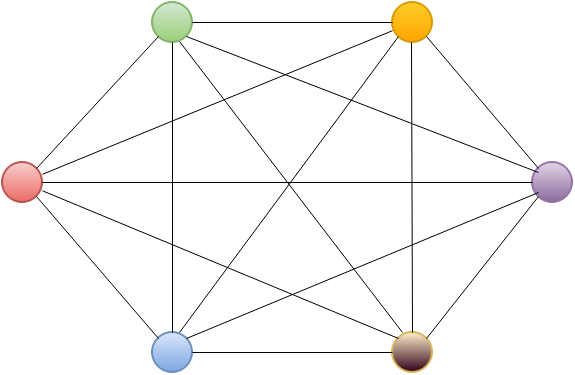
\includegraphics[scale = 0.5]{pics/clique.png}
    \caption{Clique of size $n = 6$ \label{fig:clique}}
\end{figure}
The protocol assumes that conversation participants form a clique (i.e. no two of them are strangers) and that all clique members are trustworthy (i.e. that the problem of Trust Establishment from \cref{sec:intro.overview_sec_mess} has already been solved via other means). 


\subsection{Clique formation}
\label{subsec:prep.formation}
Every clique has a \emph{common secret} that all participants share and which is regularly updated. When a clique is started, members are added one-by-one. One of the members first creates a singleton clique with a random secret, and then adds other participants. To add a user, one of the clique members performs a Diffie-Hellman key exchange \cite{diffie1976new} with the them, using the current clique secret as the secret exponent, thereby negotiating a new common secret based on the previous one. When other clique members are notified of the new user, they also update their version of the secret. 

Diffie-Hellman is a key exchange protocol that allows two parties to establish a common secret over an insecure channel. It uses two fixed publicly known parameters $G$ and $P$, such that $G$ is a generator of the cyclic group of order $P$. Let's say user Alice is a member of an existing clique with common secret $s$, and she wants to invite user Bob to the conversation. 
\begin{figure}[h]
    \captionsetup{width=0.8\textwidth}
    \centering
    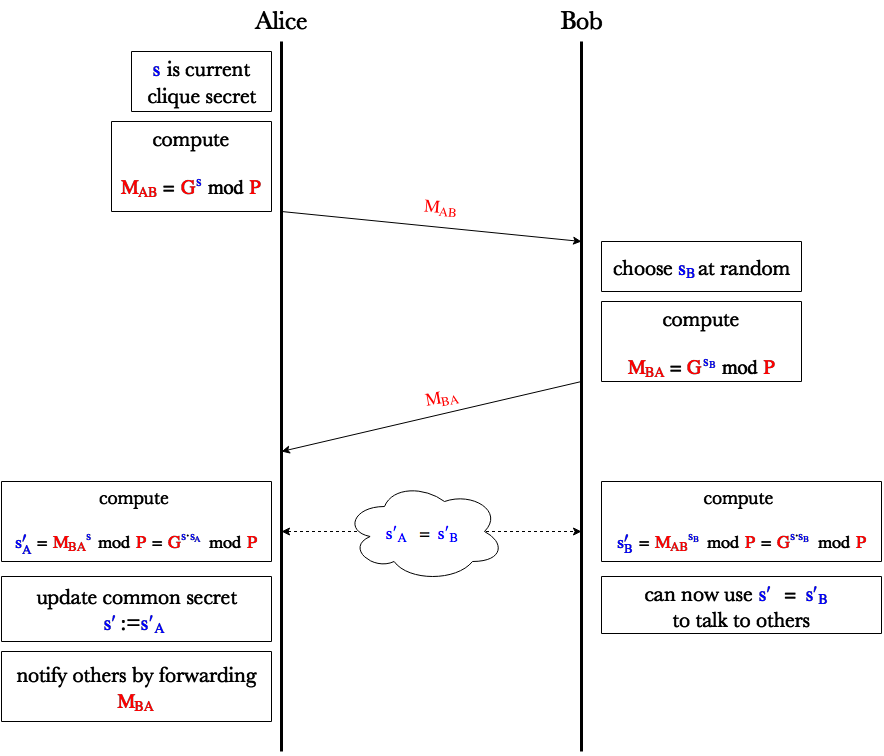
\includegraphics[width = 0.85 \linewidth]{pics/DH.png}
    \caption{Adding a new user to an existing clique using Diffie-Hellman key exchange. Public information is in {\color{red}red}, secret -- in {\color{blue}blue}.}
    \label{fig:DH}
\end{figure}

She sends Bob the modular exponent $M_{AB} = G^{s} \bmod P$. Upon receiving this message, Bob generates a random number $s_B$ and sends Alice $M_{BA} = G^{s_B} \bmod P$. Bob now computes $s'_B = M_{AB}^{s_B} \bmod P = G^{s \cdot s_B} \bmod P$. When Alice receives Bob's response, she computes $s'_A = M_{BA}^{s} \bmod P = G^{s \cdot s_B} \bmod P$ and updates the clique's common secret to be this new value. Clearly, $s'_A = s'_B = s'$, so Bob now also knows the secret and can use it to participate in the conversation. \\

An adversary who can observe this exchange and see both $M_{AB}$ and $M_{BA}$ has no computationally feasible way to determine the values of $s$ and $s_B$ and cannot compute the common secret $s' = G^{s \cdot s_B}$. The security of Diffie-Hellman relies on the difficulty of the Discrete Logarithm Problem in the chosen cyclic group, so it makes sense to choose parameters $G$ and $P$ to be very large. It is also worth pointing out  that this scheme is clearly vulnerable to a man-in-the-middle attack where an active adversary modifies the values of $M_{AB}$ and $M_{BA}$, essentially impersonating each user to the other one. This can be solved by some form of authentication, but this problem belongs to the realm of Trust Establishment (\cref{sec:intro.overview_sec_mess}) and is therefore outside the scope of KleeQ.


\subsection{Exchanging messages}
\label{subsec:prep.patching}
Clique members exchange messages through the procedure of \emph{patching}. This process needs two pieces of information that each user maintains -- the current \emph{transcript} of the conversation and the \emph{version vector}. The version vector is a vector of same size as the clique, where each entry corresponds to the number of messages authored by a particular conversation participant. The \emph{patching algorithm} is then as follows: \\ 
\begin{algorithm}
\caption{The Patching Algorithm}
\label{alg:patching}
{\bfseries Alice}
\begin{enumerate}
    \item Sends her version vector $v_A = (v_{A1}, v_{A2}, ..., v_{An})$ to Bob. \\
\end{enumerate}

{\bfseries Bob}
\begin{enumerate}
    \item Calculates the difference between his own version vector and the one sent by Alice, to see what messages she is missing:
        \begin{equation*}
            v_{\Delta} = v_B - v_A
        \end{equation*}
    \item {Generate a patch to provide the missing messages: \newline \vspace{-5mm}}
        \begin{algorithmic}
            \STATE \textit{Patch} $\leftarrow \emptyset$
            \FOR{$i$ from $1$ to $n$}
                \IF{$v_{\Delta i} > 0$}
                    \STATE \textit{Patch.add}(last $v_{\Delta i}$ messages authored by participant $i$)                        
                \ENDIF
            \ENDFOR
        \end{algorithmic}
    \item Send the \textit{Patch} and version vector $v_B$ to Alice. \\
\end{enumerate}

{\bfseries Alice}
\begin{enumerate}
    \item Insert the messages provided by Bob into transcript.
    \item As above, compute difference between $v_A$ and $v_B$, to see what messages Bob is missing.
    \item As above, generate a \textit{Patch} and send it to Bob. \\
\end{enumerate}

{\bfseries Bob}
\begin{enumerate}
    \item Insert the messages provided by Alice into transcript.
\end{enumerate}
\end{algorithm}

The above exchange happens regularly between every pair of clique members, and makes sure that their views of the transcript contain the same messages. \\

In order to ensure identical \emph{ordering} of messages in the clique, each participant also maintains a \emph{Lamport timestamp} which is initially set to 0. When two users patch each other as shown above, they update their timestamps to one plus the maximum of their Lamport times. Every time a message is written, it is given the current Lamport time of the author which is then incremented by one. We can thus define a \emph{total order} $<_L$ on messages as follows:\\

\[
    <_L(m_1, m_2) = 
        \begin{cases}
            \mathtt{TS}(m_1) < \mathtt{TS}(m_2) & \mathtt{TS}(m_1) \neq \mathtt{TS}(m_2) \\
            <_{lex}(\mathtt{Author}(m_1), \mathtt{Author}(m_2)) & \text{otherwise}
        \end{cases}
\] \\

where $\mathtt{TS}$ is the Lamport timestamp of a message and $<_{lex}$ is lexicographic comparison of authors' names. The $<_L$ relation allows the clique members to arrange all messages in a linear sequence, sorting them by Lamport time and breaking ties by comparing the names of authors lexicographically. \\ 

It can be formally proven \cite{reardon2007kleeq} that exchanging messages as specified by Algorithm \ref{alg:patching} and ordering them using the $<_L$ relation results in all participants converging on the same version of the transcript.


\subsection{Transcript verification}
\label{subsec:prep.sealing}
In an ideal situation, just using the scheme above will allow the clique to converge on the correct single transcript. However, in the more realistic setting where network errors can occur or a malicious adversary can try to inject fake content, measures must be taken to verify the \emph{integrity} of the conversation. In other words, it is necessary to make sure that all users have the same view of the conversation. This is done using the process of \emph{block sealing}. \\

In brief, the scheme involves the clique members independently dividing the transcript into blocks in a deterministic fashion and \emph{sealing} them by comparing the hashes of their content. For this to work correctly, it is necessary to choose blocks to be sealed in a way which would guarantee that all messages in them have been received and none are missing. This task is performed by the \emph{block finding algorithm} (Algorithm \ref{alg:block_find}). \\

Intuitively, in Stage 1 the algorithms scans the unsealed part of the transcript (its \emph{tail}) backwards, starting with most recent messages, until it has seen at least one message authored by each of the clique members. Because of how the patching algorithm works, it is certain that the remaining, less recent part of the transcript (also referred to as the \emph{sealable set}) contains no missing messages. In Stage 2, blocks are extracted from the sealable set by scanning it in chronological order and taking the smallest message subsequence in which every user has authored at least one message. There is a formal proof \cite{reardon2007kleeq}, omitted here for brevity, that this algorithm allows the clique members to compute identical blocks independently. {\color{red} Pic to illustrate this?}\\

Every block is given a sequential number. When a block is found, the concatenation of its sequential number and its messages are hashed to compute the \emph{fingerprint} of the block, which the clique members then verify with each other. After verification, the sealed blocks are \emph{safely deleted}, which is partly how forward secrecy is achieved.

\begin{algorithm}
\caption{The Block Finding Algorithm}
\label{alg:block_find}
\textbf{Input}
\begin{itemize}
    \item $C$: clique
    \item $M$: sequence of unsealed messages (\emph{tail}) \\
\end{itemize}

\textbf{Output}
\begin{itemize}
    \item $B$: prefix of $M$ which is a sealable block, or $\emptyset$ if no such block can be found \\
\end{itemize}

\textbf{Variables}
\begin{itemize}
    \item SeenSet: set of uniquely seen authors
\end{itemize}


\textbf{Procedure}
\vspace{3mm}
\begin{algorithmic}
    \STATE \textbf{\textit{Stage 1: calculating the sealable set \vspace{3mm}}}
    \STATE
    \begin{enumerate}
            \STATE SeenSet $\leftarrow \emptyset$
            \begin{spacing}{1.2}
            \FOR{$i$ from $|M|$ down to $1$}
                \STATE $m \leftarrow M[i]$
                \STATE $SeenSet \leftarrow SeenSet \cup \{Author(m)\}$
                \IF{$|SeenSet| = |C|$}
                    \STATE $S \leftarrow M[1..i]$
                    \STATE \textbf{break}
                \ENDIF
            \ENDFOR
            \IF{$|SeenSet| \neq |C|$}
                \RETURN $\emptyset$
            \ENDIF
            \end{spacing}    
    \end{enumerate}
    \STATE \textbf{\textit{Stage 2: finding a block \vspace{3mm}}}
    \begin{enumerate} \setcounter{enumi}{3}
        \STATE SeenSet $\leftarrow \emptyset$
        \begin{spacing}{1.2}
        \FOR{$i$ from $1$ up to $|S|$}
            \STATE $m \leftarrow S[i]$
            \STATE $SeenSet \leftarrow SeenSet \cup \{Author(m)\}$
            \IF{$|SeenSet| = |C|$}
                \RETURN $S[1..i]$
            \ENDIF
        \ENDFOR
        \end{spacing}
        \vspace{-2mm}
        \RETURN $\emptyset$
    \end{enumerate}

\end{algorithmic}


\end{algorithm}
\subsection{Key management}
\label{subsec:prep.keyman}
As described in \cref{subsec:formation}, each clique has a common secret. This secret is used to derive the \emph{key} which is then used to encrypt and authenticate the communication. The secret and the key are updated on multiple occasions. Initially, the key is calculated as:
\begin{equation*}
    k \leftarrow MAC_{s}(cliqueName)
\end{equation*}
where $s$ is the initial random secret and $cliqueName$ is the public name of the clique that is known to all participants. \\ 

When a new participant is added, the secret gets renegotiated as per \cref{subsec:prep.formation}, and the key is also recomputed: \\
\[
    s_{i+1} \leftarrow G^{s_i \cdot s_{other}} \bmod P  \\ 
\]
\[
    k_{i+1} \leftarrow MAC_{s_{i+1}}(cliqueName)
\] \\


The key also gets rotated when a block is sealed:
\[
    s_{i+1} \leftarrow MAC_{k_i}(s_i) \\ 
\]
\[
    k_{i+1} \leftarrow MAC_{s_{i+1}}(block\_content)
\] \\

The resulting chain of secrets and keys can be schematically summarised as follows:
{ 
    {\color{red} Schamatic pic here!}
} \\ 
Note that the key rotation scheme helps us achieve both forward and backward secrecy. Given a compromised key, extracting the previous one is essentially equivalent to online inversion of a hash function, whereas computing the next key in the chain would require the adversary to also know the current secret.


\subsection{Message Format}
\label{ssec:prep.proto.msg_fmt}
Another issue that we need to solve is addressing. When a KleeQ instance receives an encrypted message, it needs to determine which clique it belongs to. This is done using \emph{address tags}, which is something that each clique has at all times. It is always equal to:
\begin{equation*}
    c_{id} = MAC_{k}(cliqueName)
\end{equation*} \\
This tag is at the beginning of every transmission and in conjunction with a look-up table of address tags can be used by a KleeQ instance to demultiplex messages into appropriate cliques as they arrive. As keys are rotated, old address tags are removed from the look-up table and new ones are added.\\

In addition, to protect the content of the communication from being viewed and/or modified by the adversary, we need to encrypt and authenticate all messages using the current clique key. Following the recommended practices, we first encrypt the message and then MAC the concatenation of the ciphertext and the clique name. This allows to discard messages if they do not pass integrity checks, without attempting to decrypt them first.

Eventually, for a message $m$ we transmit the following:
\begin{equation*}
    T = c_{id} || E_k(m) || MAC_k(cliqueName || E_k(m))
\end{equation*}
Replay attacks are prevented by each $m$ containing the name of the author, name of the recipient and the sender's Lamport time.

\section{Requirements Analysis}
\label{sec:prep.requirements}
The requirements for the project follow directly from the aims outlined in \cref{sec:intro.aims} and success criteria mentioned in the proposal\footnote{See Appendix \ref{appendix:proposal}}. They can be summarised as follows:
\begin{description}[labelindent=0.5cm, leftmargin=1.3cm, rightmargin=0.5cm]
    \item[Implementing the protocol] \hfill \\
        Implement the protocol exactly as specified in \cref{sec:prep.proto}, ensuring that all of its security guarantees still hold, namely:
        \begin{itemize}
            \item confidentiality of message content
            \item message integrity
            \item forward secrecy
            \item backward secrecy
            \item message authorship repudiation
            \item conversation participation repudiation
        \end{itemize}


    \item[Construct a useable messaging application] \hfill \\
        Build a simple messaging application based in our protocol implementation.     
\end{description}
It is worth pointing out that these two items are mutually dependent -- implementing and debugging the protocol requires some kind of messenger prototype to be in place. This circumstance was identified early on and taken into account when planning the work (\cref{sec:prep.impl_strat}). \\


\section{Preliminary System Design}
\label{sec:prep.design}
Some early architecture design was done before any code was written. In particular, the main classes of the implementation were conceived and thought through, and some of the additional external components necessary for operation of the protocol were engineered.
\subsection{Secondary components}
In order to implement and run KleeQ, it was necessary to address some secondary practical issues first. These issues are:
\begin{description}[labelindent=0.5cm, leftmargin=1.3cm, rightmargin=0.5cm]
    \item[Contact Discovery] \hfill \\
        How do we know where our peers reside? Which IP-addresses do we send messages to?
    \item[Transport] \hfill \\
        How do we send messages to peers are not publicly addressable on the Internet? What if they have a non-pubic IP-address (e.g. if they are behind a NAT)?
\end{description}

Both of these issues can be solved in a completely distributed fashion in a ``pure'' P2P way (e.g. using distributed hash tables), but in order to meet the time constraints of this project it was decided to use a centralised server-based solution. \\

For the purpose of running KleeQ two server ``scaffolding'' applications were designed:
\begin{description}[labelindent=0.5cm, leftmargin=1.3cm, rightmargin=0.5cm]
    \item[Address Book]\hfill \\
        This component keeps track of users' IP-addresses. All KleeQ instances perform a \emph{check-in} every once in a while, thereby updating the records in the address book. 
        \begin{figure}[H]
            \centering
            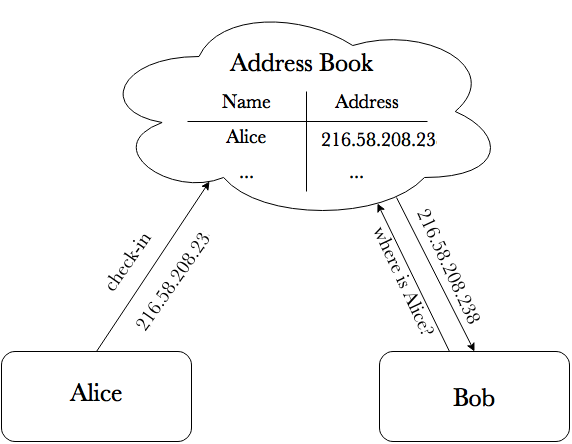
\includegraphics[width = 0.6 \linewidth]{pics/addressBook.png}
            \caption{\label{fig:addressBook}Operation of the Address Book}
        \end{figure}
        Other users query the address book when they need to send a message, and get the current IP-address of the destination.

    \item[Store-and-Forward Service] \hfill \\
        This application is used as a relay station to leave messages to be collected by other users later. It operates as a collection of ``pigeonholes'' where users put messages when they want to communicate and which are emptied by recipient every once in a while. 
        \begin{figure}[H]
            \centering
            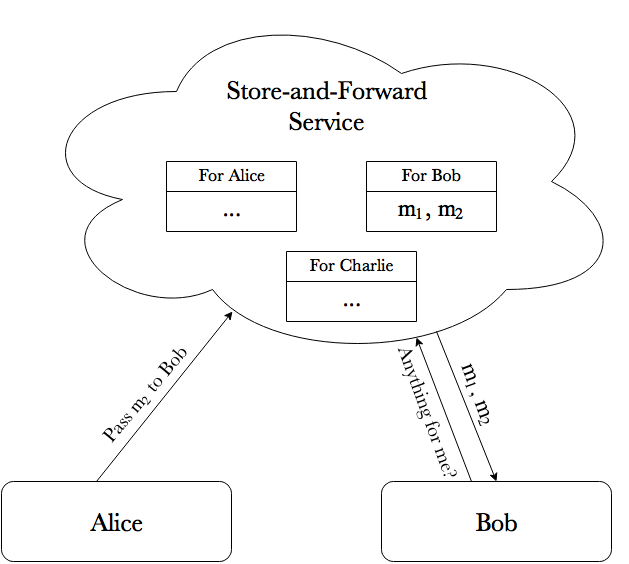
\includegraphics[width = 0.6 \linewidth]{pics/saf.png}
            \caption{\label{fig:addressBook}Operation of the Store-and-Forward Service}
        \end{figure}
        This scheme allows communication between users who do not have public IP-addresses, since the connection to the store-and-forward is always initiated by the client.
\end{description}


\subsection{Object-oriented design}
In order to make writing code easier, a rough object-oriented design of the core part of the client application was produced. It consists of the three most important classes -- Communicator, Client and Clique.

\begin{figure}[H]
    \centering
    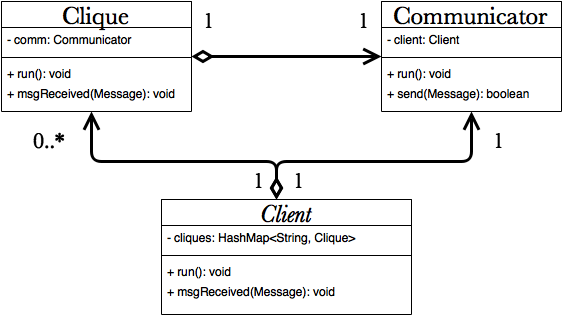
\includegraphics[width = 0.7 \linewidth]{pics/core_uml.png}
    \caption{\label{fig:core_uml} Core part of the client application}
\end{figure}

Each of these three classes are \emph{active}, i.e. they are running as separate threads. Communicator is in charge of sending and receiving messages (directly via TCP or via Store-and-Forward). When a message is received, the Communicator gives a callback to class Client which demultiplexes the message into the appropriate Clique (as specified in \cref{ssec:prep.proto.msg_fmt}) by redirecting the callback to it. Class Clique is responsible for performing most of the actual protocol (as per \cref{sec:prep.proto}), including patching, sealing, key management etc. When Clique needs to send a message, it uses the Communicator for this. Apart from re-directing messages to the right cliques, the Client class is also handing the interaction with the user (e.g. command-line interface or GUI).

\section{Implementation Strategy}
\label{sec:prep.impl_strat}
It became clear early on that before commencing the implementation of the actual protocol the following preparatory steps needed to be taken:
\begin{itemize}
    \item Building and testing the ``scaffolding'' server components, i.e. the Address Book and the Store-and-Forward.
    \item Implementing the transport functionality on the client side (class Communicator in Figure \ref{fig:core_uml}).
    \item Preparing a simple command-line interface to be able to test different parts of the code without changing it (part of class Client in Figure \ref{fig:core_uml}).
\end{itemize}

Given the small size and relatively low complexity of the tasks above, it was decided to implement these parts of the project following the \emph{waterfall model} -- do the design work upfront and write the code to fit the specifications. \\

Implementing KleeQ itself required a more flexible approach and the \emph{iterative model} was chosen. The plan was to produce a series of prototypes, adding features incrementally:
\begin{description}[labelindent=0.5cm, leftmargin=1.3cm, rightmargin=0.5cm]
%    \item[Prototype 0: Basic Communication]\hfill \\
%        Send strings back and forth between two instances of the program through Store-and-Forward and directly via TCP. Make sure all the preparatory code is functioning properly.
    \item[Prototype 1: Clique Formation]\hfill \\
        Implement clique formation (\cref{subsec:prep.formation}). Make sure users compute the shared secret correctly. Add encryption and authentication.
    \item[Prototype 2: Patching]\hfill \\
        Instead of sending messages directly, use the patching algorithm (\cref{subsec:prep.patching}). Make sure users converge on a single transcript.
    \item[Prototype 3: Sealing]\hfill \\
        Verify the global transcript via the process of block sealing (\cref{subsec:prep.sealing}). Make sure the blocks are calculated, verified and deleted correctly.
    \item[Prototype 4: Key Management]\hfill \\
        Improve key management by implementing key rotation (\cref{subsec:prep.keyman}). Make sure rotation of address tags (\cref{ssec:prep.proto.msg_fmt}) does not disrupt communication.
    \item[Prototype 5: Interface] \hfill \\
        Enhance user interaction by building a GUI. Prepare for automated evaluation by constructing a ``machine interface'' for use by testing scripts. 
\end{description}

\section{Choice of Technology, Libraries and Tools}
The technology and libraries were carefully chosen so as to make the development process more smooth, as well as to allow for some flexibility and modularity.

\subsection{Server side}
Server-based components were implemented in Python, using the RESTful HTTP framework called Flask\footnote{\url{http://flask.pocoo.org}}. For the purpose of running the code, a cloud server was rented from the PaaS provider PythonAnywhere\footnote{\url{https://www.pythonanywhere.com/}}. As noted before, most of the server-side development needed to be done before writing any client code, so the testing was performed manually, using a simple utility called Postman\footnote{\url{https://www.getpostman.com/}} which allows sending custom HTTP requests and receive responses. Programming in Python was done in PyCharm IDE.

\subsection{Client side}
The client-side code was written in Java, using the IntelliJ IDE. Messages were serialised into JSON strings using the json.simple\footnote{\url{https://github.com/fangyidong/json-simple}} library. The graphical interface was built using the Swing framework. The project relied on \texttt{git} for VCS, and the back-up strategy involved regular uploads to GitHub and copying to an external hard drive.

\section{Summary}
This chapter has described the KleeQ protocol in full detail (\cref{sec:prep.proto}), presented the formal requirements for this project (\cref{sec:prep.proto}), familiarised the reader with the early design work (\cref{sec:prep.design}) and the planning (\cref{sec:prep.impl_strat}) that was performed before any code was written. The next chapter provides further detail of design and elaborates on some interesting aspects of the implementation.



\chapter{Implementation}
{\color{red} Roadmap?}
\section{Preparatory coding}
As explained in the previous chapter, implementing KleeQ as described in \cref{sec:prep.proto} required some other code to be written first. In particular, the following components needed to be built and tested:
\begin{itemize}
    \item server Python applications (Address Book and Store-and-Forward)
    \item client-side code for interacting with the server
    \item a command-line interface (CLI) for basic group chat operations
\end{itemize}
The next few sections describe in detail how these tasks were performed.

\subsection{Server-side applications}
This part of the work was regarded as a necessary diversion from the original goal of implementing and evaluating KleeQ, and therefore the design decisions were directed towards simplicity and quickness of implementation. Both server components are small HTTP services -- the choice of protocol has been motivated by a good selection of third-party libraries for HTTP communication and the fact that it usually is not blocked by firewalls.\\

The Address Book and the Store-and-Forward (SaF) service were implemented using Flask, a RESTful Python framework for building HTTP server applications. Essentially, it provides an easy and efficient way to write server code which accepts and replies to HTTP requests. Here is a quick example of how it works: \\

\begin{lstlisting}[language = Python, columns=fullflexible]
from flask import Flask
app = Flask(__name__)

@app.route("/hello/<userID>")
def welcome(userID):
    return "Hello and welcome, %s!\n" % (userID)
    
if __name__ == "__main__":
    app.run()
\end{lstlisting}


The framework allows to define callback functions which get invoked when an HTTP request is received for a particular URL. For example, if the program above were running on \url{www.example.com} (on port 80), then typing \url{www.example.com/hello/Pavel} into the browser would result in the function above being called and the text "Hello and welcome, Pavel!" displayed. \\

Any complex server behaviour can be achieved in a similar way. This kind of system design is called \emph{Representational State Transfer} (REST) -- requests are encoded as access requests for some resource.  All functions of our server applications are defined in this RESTful way -- they are callbacks whose invocation is triggered by HTTP requests for specific URLs, which makes the code very easy to debug using a browser.

\subsubsection{Address Book}
This application is essentially an online look-up table which is used by client applications to record their \emph{network addresses} (IP-address and port) from time to time (\emph{"check-in"}), so that their peers knew where to send messages for them. The service has 3 commands:

\begin{table}[H]
\centering
\begin{tabular*}{0.9\textwidth}{l | c | l}
    Command & Arguments & Function \\
    \hline
    check-in & userID, IP:port& Records address of a particular user \\
    lookup & userID & Returns the address of a given user \\
    display & --  & Returns addresses of all known users \\
\end{tabular*}
\caption{\label{tab:address_book} Functionality of the Address Book}
\end{table}

All of these commands are defined as Flask callback, similar to the example above. The implementation is based on a hash map (or dictionary, in Python parlance) which maps unique user names (\emph{userIDs}) to network address strings. When a user checks-in, their record is updated. In addition, every record contains the time of last check-in which is used to clear out stale records as users go offline. If a check-in happens from an IP-address belonging to the private range, then the system records it as "0.0.0.0:0", which serves as a signal for everyone that this user cannot be reached directly and all communication with them should be happening through the store-and-forward service.

\subsubsection{Store-an-Forward}
The operation of this component is analogous to that of a pigeonhole area at a Cambridge college. Users leave their communications (encrypted or otherwise) in ``pigeonholes'' marked with unique userIDs which are regularly emptied by their owners. The purpose of this arrangement is to facilitate communication in cases when a direct TCP connection cannot be easily made (e.g. when the destination resides behind a NAT). Table \ref{tab:saf} presents the function set of the service.

\begin{table}[H]
\centering
\begin{tabular*}{0.9\textwidth}{l | c | l}
    Command & Arguments & Function \\
    \hline
    store & userID, msg & Stores a message for a given user \\
    retrieve & userID & Returns all messages for user, clears postbox\\
    view & userID & Returns all messages for a specific user \\
\end{tabular*}
\caption{\label{tab:saf} Functionality of the Address Book}
\end{table}

As before, each command is implemented as a Flask callback procedure. The implementation is based on a hash map where userIDs are keys and lists of base64-encoded message strings are values.


\subsection{Client-side API for server applications}
As mentioned before, the server applications use HTTP to communicate with the outside world. To access the commands of the services from the client application, a Java API has been built. It is a collection of static methods contained in 3 classes, which provide a convenient interface to the server components by sending the appropriate HTTP requests.

\begin{figure}[H]
    \centering
    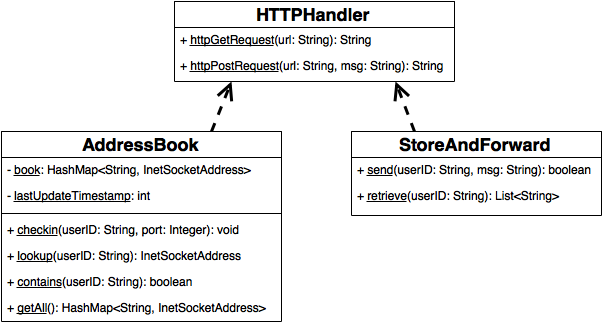
\includegraphics[width = 0.8 \linewidth]{pics/scaffolding_uml.png}
    \caption{\label{fig:scaffolding_uml} Class diagram of the API to server components}
\end{figure}
In Figure \ref{fig:scaffolding_uml}, class HTTPHandler implements the functionality for sending HTTP GET and POST requests. These two methods are used by classes AddressBook and StoreAndForward to access the commands of the server applications. The rest of the client-side code can therefore use these classes to communicate with the server components as if they were available locally (\emph{access transparency}). \\

In an early implementation of the AddressBook class, the methods \texttt{lookup()} and \texttt{contains()} were sending an HTTP request to the server upon every invocation which considerably slowed down the whole program. To solve this problem, a simple \emph{caching system} was built-in -- the class downloads the whole address book from the server every few seconds, and the methods use this downloaded copy to compute their results. This means that the methods may return results that are slightly stale, but this does not cause any issues for KleeQ due to its inherently asynchronous nature. \\

%Each client instance contains an \emph{address-reporting thread} which calls the \texttt{checkin()} method from time to time, to update the server records about itself.

\subsection{Client-side transport code}
The interface described above is primarily used by the Communicator class (see Figure \ref{fig:core_uml}), which is responsible for transport and connectivity. The class contains three threads that are perpetually running:
\begin{description}[labelindent=0.5cm, leftmargin=1.3cm, rightmargin=0.5cm]
    \item[Address-reporting thread] \hfill \\
        Calls the Address Book \texttt{checkin()} method every few seconds, to update/renew the server records about the address of the client. If the Address Book is unreachable then the client assumes it is offline.
    \item[SaF Querying Thread] \hfill \\
        Calls the StoreAndForward \texttt{retrieve()} function every few seconds, and gives a callback to the Client class for each of the new messages.
    \item[TCP Socket Server Thread] \hfill \\
        Listens on a port (randomly chosen at start up) for direct TCP connections, also giving callbacks to the Client class as messages arrive.
\end{description}
At this point, the reader may be wondering why threads for \emph{both} direct TCP transmission and for SaF run at the same time. Indeed, as of now communication happens only though one of the two -- it is direct (via TCP) if the client is running on a public IP-address, and via SaF otherwise. However, it is worth noticing that it may be possible to connect two client directly even when they are not publicly addressable if they happen to reside on the \emph{same local network}. This feature has not been implemented so far, but would definitely be useful in the future. \\

\begin{figure}[H]
\centering
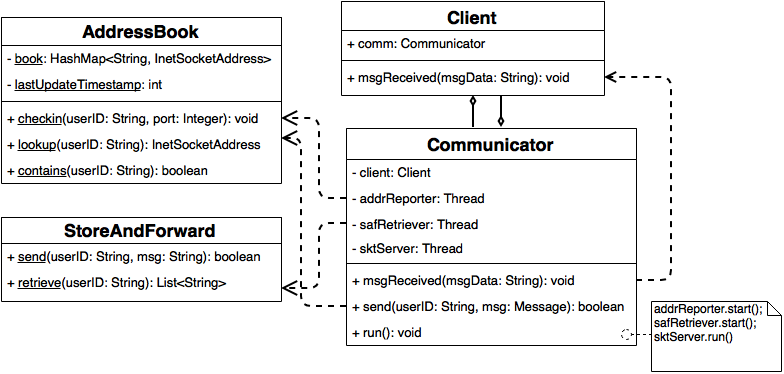
\includegraphics[width = 0.8 \linewidth]{pics/communicator_uml.png}
\caption{\label{fig:communicator_uml} Operation of the Communicator class}
\end{figure}


The Communicator class also contains a \texttt{send()} method which uses the data in the Address Book to decide which of the two transport options (direct TCP or SaF) to use for the given destination, and sends the message. The method returns a boolean value, depending on whether transmission has been successful (sending could fail e.g. if client is offline).


\subsection{A simple CLI}
The primary reason for building this component was to be able to test various aspects of the KleeQ's operation just by typing commands, without changing the source code. In addition, upfront design of a CLI helped understand what use-cases need to be handled. \\

The design involved defining a minimal set of operations that a group messaging application needs to have. The corresponding commands are shown in Table \ref{tab:CLI}.

\begin{table}[H]
\centering
\begin{tabular*}{0.9\textwidth}{l | l | l}
    Command & Arguments & Function \\
    \hline
    \multicolumn{3}{c}{\textbf{Main menu commands}} \\
    \hline
    <empty> & -- & Refresh \\
    create & groupName & Create a new group with given name \\
    add & userID, groupName & Add a specific user to a given group \\
    view & groupName & View a particular group (\emph{group view}) \\
    help & -- & Display a help message \\
    exit & -- & Terminate the program \\
    \hline
    \multicolumn{3}{c}{\textbf{Group view commands}} \\
    \hline 
    <empty> & -- & Refresh \\
    msg & msgText & Send a message to current group \\
    back & -- & Go back to main menu \\
    add & userID & Add a specific user to current group \\
    help & -- & Display a help message \\
    exit & -- & Terminate the program \\ 
\end{tabular*}
\caption{\label{tab:CLI} Command-line interface}
\end{table}
The implementation of the interface above is contained in the CLIClient class which is a subclass of Client (Figure \ref{fig:CLIClient_uml}).
\begin{figure}[H]
\centering
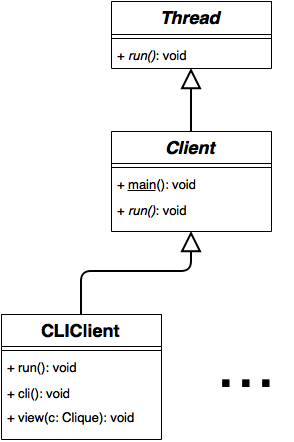
\includegraphics[width = 0.31 \linewidth]{pics/CLIClient_uml.png}
\caption{\label{fig:CLIClient_uml} The CLI is implemented in the class CLIClient}
\end{figure}
This proved to be very convenient later on, since implementing other types of interfaces (e.g. GUI) could be neatly done by creating another subclass of Client and writing a different version of the \texttt{run()} method.

The logic of the interface was coded as an infinite loop which takes keyboard input, breaks it down into terms and then tries to match them against a sequence of conditionals that correspond to different commands. If a match happens, the appropriate functions are called and relevant output is given.


\section{Protocol implementation}
Once the ``scaffolding'' (server components and CLI) was completed, it became possible to proceed with the implementation of KleeQ itself, as described in \cref{sec:prep.proto}.


\subsection{Prototype 1: Clique Formation}
Building this prototype involved implementing the procedure for creating a new clique and adding users to it. In CLI terms, it meant implementing the logic of the \texttt{create} and \texttt{add} commands. This required the following tasks to be completed:

\begin{itemize}
    \item Designing an object-oriented representation for a clique such that it neatly fits into the previous design.
    \item Working out the exact mechanics for adding a new user, based on the description in \cref{subsec:prep.formation}. Performing the necessary pieces of object-oriented design to model this process.
    \item Choosing the cryptographic methods to be used for Diffie-Hellman key-exchange, encryption and message authentication. Implementing them in the object-oriented fashion that would work well with the rest of the design.
\end{itemize}

The next few sections address these three tasks in more detail.

\subsubsection{Object-oriented clique model}
A clique is modelled by the Clique class (Figure \ref{fig:clique_uml}) which contains all the group-specific information and implements most of the protocol's logic. Instances of the class are stored in a hash map (clique name to Clique instance) contained in the Client class, and its methods are called by the UI code when the user issues a command. In addition, Client also contains a hash map that maps \emph{address tags} (\cref{ssec:prep.proto.msg_fmt}) to clique names, which is used for demultiplexing encrypted messages into destination cliques as they arrive.
\begin{figure}[H]
    %\captionsetup{width=0.8\textwidth}
    \centering
    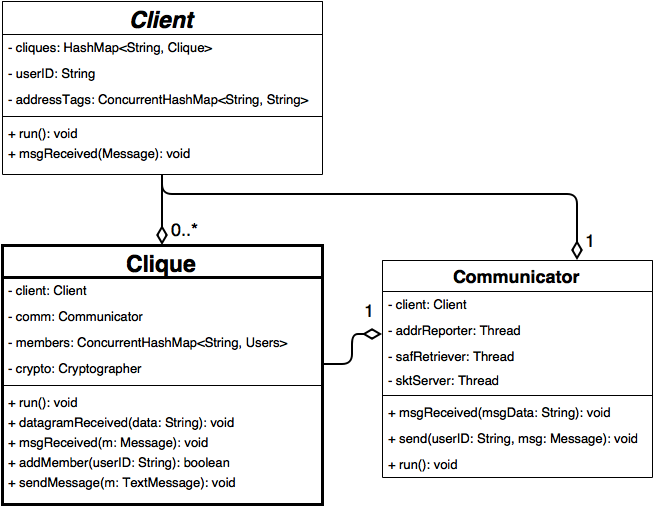
\includegraphics[width=0.8\linewidth]{pics/clique_uml.png}
    \caption{\label{fig:clique_uml} The Clique class models a communication group.}
\end{figure}

\subsubsection{Messages for adding users}
As mentioned in \cref{sec:prep.proto}, KleeQ solves the key distribution problem via the Diffie-Hellman key exchange protocol. However, apart from converging on a common secret adding a new user involves \emph{distribution of group membership information}. In other words, when a new user is added by one of the current conversation participants, they need to be notified of what \emph{other} users are part of the group. There exist multiple ways of doing it, but no particular method was suggested by KleeQ's authors in the original paper. The method that was chosen as part of this project is illustrated in Figure \ref{fig:CliqueFormation}.
\begin{figure}[H]
    \captionsetup{width=0.76\textwidth}
    \centering
    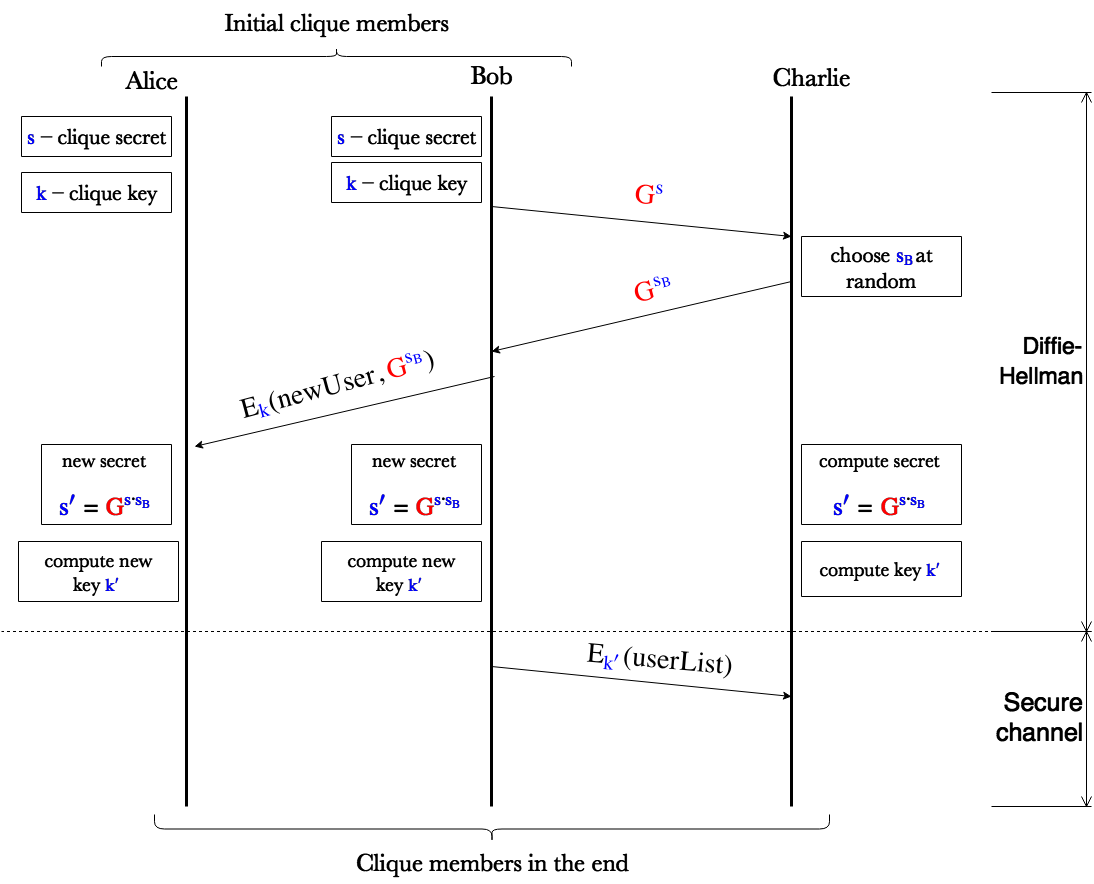
\includegraphics[width=0.76\linewidth]{pics/CliqueFormation.png}
    \caption{\label{fig:CliqueFormation} Schematic procedure for adding a new user to a clique. Public information is in {\color{red} red}, private -- in {\color{blue} blue}.}
\end{figure}
The figure shows how one of the current members (Bob) adds a new user (Charlie) to an existing clique also containing user Alice. Bob sends an invitation containing a Diffie-Hellman negotiation parameter based on the current clique secret. Charlie replies with his own negotiation parameter, and computes the new group secret and key. Upon receiving Charlie's response, Bob notifies the existing group members (Alice) of the newly added user using the \emph{old} key, also forwarding the new user's negotiation parameter. Then Bob computes the \emph{new} group secret, and uses the new key to provide Charlie with the current list of clique members ($userList = [Alice, Bob]$, in our example). \\

In terms of programming, each of the messages in Figure \ref{fig:CliqueFormation} is modelled as a Java class (see Figure \ref{fig:messages_uml}). All message classes are derived from the abstract Message parent class which contains information and behaviour common to all messages. For transmission, instances of these classes are serialised into JSON strings\footnote{Third-party json-simple library was used for this (\url{https://github.com/fangyidong/json-simple})}.

\begin{figure}[H]
    %\captionsetup{width=0.8\textwidth}
    \centering
    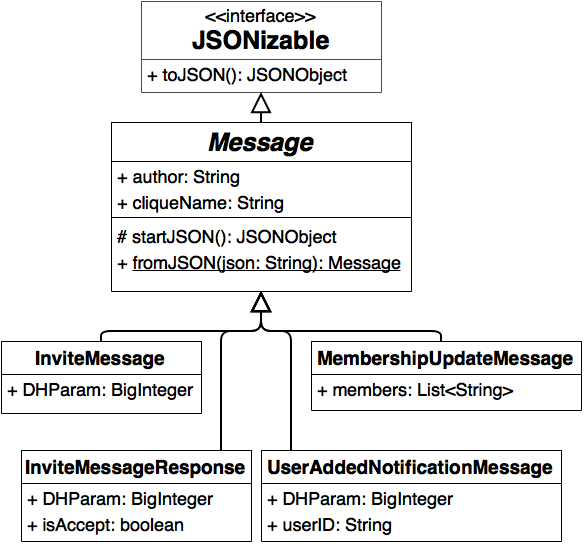
\includegraphics[width=0.6\linewidth]{pics/messages_uml.png}
    \caption{\label{fig:messages_uml} Classes modelling messages necessary to add a new user to a clique.}
\end{figure}
Conversion to JSON is performed using the \texttt{toJSON()} method, declared in the JSONizable interface and implemented in each of the child classes. When a message is received, the appropriate object is reconstructed by calling the static \texttt{fromJSON()} method in the base Message class. \\

\subsubsection{Cryptography}
The Clique class contains an instance of the Cryptographer (Figure \ref{fig:crypto_uml}) class that holds the key material and implements the relevant cryptographic procedures (Diffie-Hellman key exchange, encryption/decryption, MAC, message digest).

\begin{figure}[H]
    \captionsetup{width=0.76\textwidth}
    \centering
    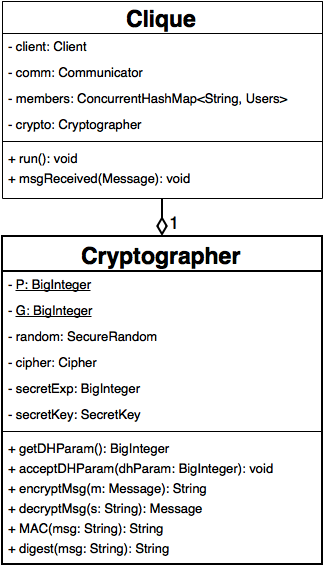
\includegraphics[width=0.4\linewidth]{pics/crypto_uml.png}
    \caption{\label{fig:crypto_uml} An instance of Cryptographer class is contained in Clique, and handles all group-specific cryptographic procedures.}
\end{figure}

The implementation of the key exchange is based on modular arithmetic with values of generator $G$ and group order $P$ taken to be:

\begin{lstlisting}[numbers=none, frame=none, xleftmargin=1.5cm, xrightmargin=0cm]

P  =  FFFFFFFF FFFFFFFF C90FDAA2 2168C234 C4C6628B 80DC1CD1
      29024E08 8A67CC74 020BBEA6 3B139B22 514A0879 8E3404DD
      EF9519B3 CD3A431B 302B0A6D F25F1437 4FE1356D 6D51C245
      E485B576 625E7EC6 F44C42E9 A637ED6B 0BFF5CB6 F406B7ED
      EE386BFB 5A899FA5 AE9F2411 7C4B1FE6 49286651 ECE45B3D
      C2007CB8 A163BF05 98DA4836 1C55D39A 69163FA8 FD24CF5F
      83655D23 DCA3AD96 1C62F356 208552BB 9ED52907 7096966D
      670C354E 4ABC9804 F1746C08 CA18217C 32905E46 2E36CE3B
      E39E772C 180E8603 9B2783A2 EC07A28F B5C55DF0 6F4C52C9
      DE2BCBF6 95581718 3995497C EA956AE5 15D22618 98FA0510
      15728E5A 8AAAC42D AD33170D 04507A33 A85521AB DF1CBA64
      ECFB8504 58DBEF0A 8AEA7157 5D060C7D B3970F85 A6E1E4C7
      ABF5AE8C DB0933D7 1E8C94E0 4A25619D CEE3D226 1AD2EE6B
      F12FFA06 D98A0864 D8760273 3EC86A64 521F2B18 177B200C
      BBE11757 7A615D6C 770988C0 BAD946E2 08E24FA0 74E5AB31
      43DB5BFC E0FD108E 4B82D120 A9210801 1A723C12 A787E6D7
      88719A10 BDBA5B26 99C32718 6AF4E23C 1A946834 B6150BDA
      2583E9CA 2AD44CE8 DBBBC2DB 04DE8EF9 2E8EFC14 1FBECAA6
      287C5947 4E6BC05D 99B2964F A090C3A2 233BA186 515BE7ED
      1F612970 CEE2D7AF B81BDD76 2170481C D0069127 D5B05AA9
      93B4EA98 8D8FDDC1 86FFB7DC 90A6C08F 4DF435C9 34063199
      FFFFFFFF FFFFFFFF
      
G  =  2
\end{lstlisting}
which is a 4096-bit group recommended for use in Internet key exchange (IKE) in RFC3526 \cite{kivinen2003more}.\\

The Diffie-Hellman procedures were implemented manually rather than using a library solution, for didactic reasons. A more advanced library implementation (e.g. based on elliptic curves) can always be easily substituted in place of the existing one if necessary -- this would only require changing the \texttt{getDHParam()} and \texttt{acceptDHParam()} methods. \\ 

For encryption, the Cryptographer uses AES -- the block cipher which seems to be the de-facto standard for symmetric encryption at the moment. We use keys of length 128 bits, as recommended by the German Office of Information Security (BSI) for use up until year 2021 \cite{margraf2016kryptographische}. Stronger cryptography (AES192 or AES256) can be enabled with almost no changes to the code (just need to change the key size constant), but this requires manual installation of the Java Cryptography Extension (JCE) which would have a negative usability effect or would necessitate the creation of an installer program. Our implementation uses AES128 in \emph{counter mode} (CTR) with the initial vector generated by a secure pseudo-random number generator. This choice was made because our messages are generally of variable length and CTR is space-efficient in this case since it requires no padding. \\

For message authentication, we use keyed-hash message authentication codes (HMAC) based on SHA256. According to a recent report by the German Office of Information Security (BSI), this cryptographic hash function can currently be considered secure and is expected to remain in active use at least until 2021 \cite{margraf2016kryptographische}. As of 2014, the best known attack could practically find a collision on 28 out of 64 rounds of SHA256 \cite{dobraunig2014analysis}. This project also uses SHA256 for computing message digests. As per the recommended practices\footnote{ISO/IEC 19772:2009}, we use encrypt-then-MAC (EtM), to not have to decrypt messages in order to verify their authenticity and integrity. \\

The same key is used for encryption and MACing. Whilst not recommended in general, this is secure in our case because we calculate:
\begin{equation*}
    MAC_k(cliqueName||E_k(m))
\end{equation*}
and there are no known interactions between AES-CTR and HMAC-SHA2. {\color{red}Correct?}

\subsection{Prototype 2: Patching}


\subsection{Prototype 3: Sealing}


\subsection{Prototype 4: Key Management}


\subsection{Prototype 5: Interface}


\chapter{Evaluation}


\chapter{Conclusions}



\bibliographystyle{unsrt}
\bibliography{bibliography}
\addcontentsline{toc}{chapter}{Bibliography}

\begin{appendices}
\chapter{Project Proposal}
\label{appendix:proposal}
\section{Introduction and Description of the Work}
\label{intro}
The recent public outcry in response to mass surveillance programs carried out by governments around the world led to creation of multiple messaging systems which emphasised security of communication. Some have been more successful than others, but each of them has been found to have some flaws or deficiencies. Broadly speaking, there are four problems that each security-oriented messenger needs to solve:
\begin{description}
    \item[Problem 1: Contact Discovery] \hfill \\
        How do we find out at which IP addresses our peers currently reside? How do we know where to send our messages?
    \item[Problem 2: Trust Establishment]\hfill \\
        Once we know where our peers are, how do we know that they are who they say they are? How do we make sure that they are not being impersonated by a malicious adversary?
    \item[Problem 3: Conversation Security]\hfill \\
        Once we are sure that we are talking to the right parties, how do we protect the security and privacy of the messages' content? In other words, how do we encrypt the messages, what data do we attach to them, and what security protocols do we perform?
    \item[Problem 4: Transport Privacy]\hfill \\
        What is the mechanics for actually sending the message so as to hide the message metadata (e.g. sender identity, recipient identity, conversation to which the message belongs etc).
\end{description}

\vspace{\baselineskip}
\noindent
Multiple protocols, with different threat definitions and varying levels of security, have been developed for each of these tasks. The aim of this project is to explore and build on KleeQ, one of the protocols aimed at providing conversation security (Problem 3 in the list above). Given a group of trusted parties residing at known addresses, it gives the following security guarantees for their conversation:
\begin{itemize}
    \item confidentiality of message content
    \item message integrity
    \item forward secrecy
    \item backward secrecy
    \item message authorship repudiation
    \item conversation participation repudiation
\end{itemize}
KleeQ has been designed for devices with transient connectivity (e.g. communication via Bluetooth or wireless), but the ideas introduced by this protocol can be used in the general setting of group messaging over a network.

\vspace{\baselineskip}
\noindent
In this project, KleeQ will be completely re-implemented into a general-purpose network conversation security protocol, preserving the security properties mentioned above. The performance characteristics will be tested, and the use of the protocol will be demonstrated by constructing a simple demo messaging app.

\vspace{\baselineskip}
\noindent
Optionally, if time allows, an attempt shall be made to make use of the most recent and secure third-party solutions to solve Problems 1, 2 and 4 from the list above, thereby producing a full-blown secure messaging application.


\section{Resources Required}
All the development will be based on the resources provided by my own machine and the PWF. In addition, it is expected that a commercial cloud hosting service (DigitalOcean, Heroku or similar) will be used, for the purpose of hosting the server side of the application. The backup strategy involves periodically pushing the code to a private GitHub repository and keeping a hand-written project log. No other resources will be required.


\section{Starting Point}
As of the starting date of the project, the following relevant background:
\begin{itemize}
    \item Experience of programming in Java, at the level of University courses \emph{Programming in Java} and \emph{Further Java}.
    \item Understanding of cryptographic primitives and computer security fundamentals, as taught in Part IB \emph{Security I} course.
    \item Limited experience of writing server-side code in Python using Flask.
\end{itemize}
\vspace{\baselineskip}


\noindent
The successful completion of the core part of the project will require the following:
\begin{itemize}
    \item Learning about the fundamentals of conversation security, understanding what security properties it entails and what the common attack strategies are.
    \item Understanding the algorithms and data structures introduced by KleeQ.
    \item Learning to write security-oriented code in Java.
\end{itemize}

\noindent
To complete the optional part, the following will need to be done:
\begin{itemize}
    \item Understanding the most common attack strategies employed by adversaries against secure messengers.
    \item Reading research papers and technical documentation describing the APIs presented by the third-party libraries in use.
\end{itemize}


\section{Substance and Structure of the Project}
\subsection{Core Part}
The core part of the project will involve re-implementing KleeQ, to make it a universal conversation security protocol. Initially, it will be necessary to obtain a deep understanding of how KleeQ operates which will be done by reading the relevant research material, as well as studying the source code of the current implementation. Then, the parts of the protocol which require re-designing to allow network communication (as opposed to ad-hoc communication via Bluetooth or similar) will be identified, and the necessary design decisions will be made. The next step will be implementing the protocol in Java and testing it locally. At that point, additional checks will be made to ensure that the new implementation retains all the security properties of the original one and, if necessary, eliminate the possible loopholes in the code.

\vspace{\baselineskip}
\noindent
The next step will be turning the result of the above into a simple desktop P2P messaging application. It is important to understand that producing a full-blown secure messaging system is outside the scope of the core part of this project -- at this stage, the aim will be to write some simple and not necessarily secure "scaffolding" code to produce a prototype, for the purposes of demonstrating the work of the new protocol implementation. In particular, it is expected that a minimalistic graphical user interface and a simple server-based contact discovery component will be implemented at this point.


\subsection{Optional Extensions}
If time allows, the most recent and secure approaches may be used to convert the aforementioned demo application into a proper secure messaging system. As mentioned in Section \ref{intro}, this would require solving the problems of secure contact discovery, trust establishment and transport privacy. These problems can be solved in the following ways:
\begin{itemize}
    \item DHT with query anonymisation for contact discovery
    \item self-auditable public key logs for trust establishment (using CONIKS)
    \item Tor-based hidden service for transport privacy and metadata hiding
\end{itemize}
All of the above are available in the form of open-source libraries which can be used in the project without major modifications.

\vspace{\baselineskip}
\noindent
In addition, an effort may be made to improve the usability of the application. With this in mind, the GUI will be refined to match the usability of the most ubiquitous messenger applications (e.g. WhatsApp, Viber, Telegram etc).




\section{Success Criteria}
There shall be two measures of success for this project:
\begin{enumerate}
    \item Implementation of a working messaging system which would be possible to use.
    \item Preservation of the security properties of the original KleeQ implementation, namely:
        \begin{itemize}
            \item confidentiality of message content
            \item message integrity
            \item forward secrecy
            \item backward secrecy
            \item message authorship repudiation
            \item conversation participation repudiation
        \end{itemize}
\end{enumerate}




\section{Timetable and Milestones}
It is important to structure the project in a way which would allow to evenly distribute the workload over the available time and minimise risks of missing deadlines. In addition, as pointed out by previous Part II students, it would be beneficial to finish the dissertation write-up at least two weeks in advance of the official deadline, to allow more time for Tripos revision. With this in mind, the following schedule has been set:


\subsection*{Weeks 1-2 (Oct 25 -- Nov 6)}
Do preliminary reading and understand the algorithms and data structures used by KleeQ, referring to the existing implementation as necessary. Identify the parts of the protocol which require modification, and design the object-oriented structure of the new implementation. Decide on which standard Java classes will need to be used. Find out what common implementation mistakes result is security loopholes. Arrange the necessary infrastructure, such as a back-up repository and cloud hosting space.

\vspace{0.7\baselineskip}
\noindent
\textit{Milestone:} The necessary knowledge of the protocol acquired, design and infrastructure ready -- can begin writing code.

\subsection*{Weeks 3-7 (Nov 7 -- Dec 11)}
Implement the protocol in Java. Test locally. Watch out for most common implementation vulnerabilities. Make sure the original security guarantees are in place.

\vspace{0.7\baselineskip}
\noindent
\textit{Milestone:} The conversation security protocol implemented and tested.

\subsection*{Weeks 9-10 (Dec 12 -- Dec 25)}
Turn the protocol implementation into a library which would be usable by third parties in their applications.

\subsection*{Week 11 (Dec 26 -- Jan 1)}
A week-long holiday is planned for these dates. No work will be done during this time.

\subsection*{Weeks 12-13 (Jan 2 -- Jan 15)}
Implement the "address book" server application to allow contact discovery. Make sure the server has the most current information about user's status. Test the practicality of KleeQ's conversation concepts.

\subsection*{Week 14 (Jan 16 -- Jan 22)}
Write-up the progress report and submit it one week ahead of the deadline.

\subsection*{Weeks 15-16 (Jan 23 -- Feb 5)}
Create a minimalistic GUI. Make sure that the cases of asynchrony (device going offline or coming back online) are adequately handled.

\vspace{0.7\baselineskip}
\noindent
\textit{Milestone:} An operational messaging application is ready. Core part of the project finished, the success criteria satisfied.


\subsection*{Weeks 17-19 (Feb 6 -- Feb 26)}
Evaluate how the protocol performs over a network under high load, and try to tune it to perform better. Refine the GUI of the prototype to allow usage by non-experts.

\vspace{0.7\baselineskip}
\noindent
\textit{Milestone:} The application looks good and the performance is satisfactory.

\subsection*{Weeks 20-21 (Feb 27 -- Mar 11)}
Implement the optional extensions as time allows. Make sure that none of the previously implemented security guarantees are broken.

\subsection*{Week 22 (Mar 12 -- Mar 18)}
A week-long holiday is planned for these dates. No work will be done during this time.

\subsection*{Weeks 23-27 (Mar 19 -- Apr 22)}
Write up the dissertation. Use the project log to recollect the details of what work has been done and how. Pay special attention to the Evaluation section, describing in detail the previously made performance measurements. Arrange regular meetings with the supervisor to receive feedback and iteratively refine the work. This part of work will take a long time, since it will be interleaved with Tripos revision over the Easter Vacation.

\vspace{0.7\baselineskip}
\noindent
\textit{Milestone:} Dissertation largely written. The supervisor and the overseers are satisfied with the content.

\subsection*{Weeks 28-29 (Apr 23 -- May 13)}
No project work is scheduled for these days -- the intention is to use this time for Tripos revision. It also provides a "safety buffer" in case more time is required, for one reason or another. If necessary, final adjustments to the text of the dissertation will be made at this time.

\vspace{0.7\baselineskip}
\noindent
\textit{Milestone:} Dissertation printed, bound and submitted at least two weeks ahead of the deadline.
\end{appendices}



\end{document}
